\documentclass[a4paper,12pt]{article}
\usepackage[fontsize=12pt]{fontsize}
\renewcommand{\baselinestretch}{1.25} 

\usepackage[margin=1in]{geometry}

\usepackage[utf8]{vietnam}
% \usepackage[vietnamese]{babel} 

\usepackage[dvipsnames, table]{xcolor} % for coloring
\usepackage{amsmath} % extension for math environment
\usepackage{bm} % bold math symbol
\usepackage{fancyvrb} % fancy verbatim
\usepackage{fvextra} % fancy verbatim extra
    \fvset{breaklines=true}

\usepackage[skip=.5em]{caption} % adjust spacing between figure and caption
\usepackage{subcaption}

% \usepackage[pdftex]{graphicx}
% \usepackage{url} 
\usepackage[bookmarks, 
    colorlinks=false, 
    pdfborder={0 0 0}, 
    pdftitle={Báo cáo BTL Xử lý số tín hiệu}, 
    pdfauthor={Phạm Khánh}
]{hyperref} 

\usepackage{tikz} 
\usetikzlibrary{calc} % for drawing rectangle box at the cover

% FOR TABLE:
\usepackage{tabularx}
    \newcolumntype{L}[1]{>{\raggedright\arraybackslash}p{#1\textwidth}}
    \newcolumntype{C}[1]{>{\centering\arraybackslash}p{#1\textwidth}}
    \newcolumntype{R}[1]{>{\raggedleft\arraybackslash}p{#1\textwidth}
} % custom table environment
\usepackage{multirow}
\renewcommand{\arraystretch}{1.2}
\usepackage{longtable}

\usepackage{enumitem} % adjusting enum and itemize environment
    \setlist[itemize]{itemsep=0pt, topsep=3pt} % no item separation
    \setlist[enumerate]{itemsep=0pt, topsep=3pt} 
\usepackage{float} % forcing figure environment to be placed at an exact location

\setlength{\parskip}{0.5em} % spacing between paragraphs
\setlength\parindent{0pt} % do not indent the first paragraph

\usepackage{listings} % for embedding code
\lstset{frame=tb,
  aboveskip=5mm,
  belowskip=5mm,
  showstringspaces=false,
  columns=flexible,
  % basicstyle={\small\ttfamily},
  basicstyle={\ttfamily},
  lineskip={.1em}, % in case line spacing is too wide
  % numbers=none,
  numberstyle=\tiny\color{blue},
  keywordstyle=\color{red},
  commentstyle=\color{pink},
  stringstyle=\color{green},
  breaklines=true,
  breakatwhitespace=true,
  tabsize=4, 
  numbers=left,
  frame=single
}

\lstdefinestyle{output}{
    basicstyle={\small\ttfamily},
    numbers=none,
    frame=none
}

\usepackage{biblatex}
\addbibresource{refs.bib}

\begin{document}
% \renewcommand{\bibname}{Tài liệu tham khảo} % For books, reports
\renewcommand{\refname}{Tài liệu tham khảo} % For articles
\renewcommand{\listfigurename}{Danh sách hình minh họa}

\begin{titlepage}
    \begin{tikzpicture}[remember picture, overlay]
        \draw[line width = 4pt] ($(current page.north west) + (.75in,-.75in)$) rectangle ($(current page.south east) + (-.75in,.75in)$);
    \end{tikzpicture}
    
    \begin{center}
    	\textbf{ĐẠI HỌC QUỐC GIA THÀNH PHỐ HỒ CHÍ MINH}\\[3pt]
    	\textbf{TRƯỜNG ĐẠI HỌC BÁCH KHOA}\\ 
    	
    	\vspace{1.5cm}
    	
\includegraphics[width=4cm]{../images/logo_BK.png}
    	\vspace{0.5cm}
    \end{center}
    
    \begin{center}
        \setlength{\parskip}{.5em}
        \par\noindent\rule{0.8\textwidth}{0.4pt}

        \textbf{{MÔN HỌC: XỬ LÝ SỐ TÍN HIỆU (EE2015)}}
        
        \textbf{{\large BÁO CÁO BÀI TẬP LỚN}}
    	    
        \textbf{{GIẢM NHIỄU HÌNH ẢNH BẰNG RASPBERRY PI 3}}
        \par\noindent\rule{0.8\textwidth}{0.4pt}
    \end{center}
    
    \vspace{1em}
    \begin{center}
        \renewcommand{\arraystretch}{1.5}
        \begin{tabular}{R{0.35} L{0.3} L{0.25}}
            \textbf{Giảng viên hướng dẫn:} & GS. TS. Lê Tiến Thường\\
            \textbf{Sinh viên thực hiện:} & Phạm Khánh & MSSV: 2011391\\
            & Lê Vĩnh Hưng & MSSV: 2010305\\
            \textbf{Nhóm} & P01 -- Nhóm 2 & 
        \end{tabular}
    \end{center}
    
    \vfill
    \begin{center}
        Tp. Hồ Chí Minh -- 2024
    \end{center}
    \vspace{1em}
\end{titlepage}

\pagenumbering{roman}
\tableofcontents

\newpage
\pagenumbering{arabic} 

\section{Giới thiệu}

Lĩnh vực hình ảnh kỹ thuật số luôn phải đối mặt với một thách thức dai dẳng: nhiễu hình ảnh. 
Sự thay đổi không mong muốn về độ sáng hoặc màu sắc này xuất phát từ các yếu tố như hạn chế của cảm biến hoặc điều kiện ánh sáng yếu, có thể che khuất các chi tiết và làm giảm độ trung thực của hình ảnh. 
Do đó, đề tài này đề cập đến các kỹ thuật giảm nhiễu hình ảnh thực hiện trên phần cứng Raspberry Pi 3. 

Đề tài này có ứng dụng thực tiễn cao vì hai mục đích chính. 
Đầu tiên, ảnh số hiện rất phổ biến trong nhiều lĩnh vực khác nhau như nhiếp ảnh, ảnh y tế, hệ thống giám sát... và nhiễu luôn là một vấn đề lớn.
Thứ hai, các phần cứng nhúng ngày càng phổ biến và có giá thành rẻ hơn, cùng với sức mạnh tính toán ngày càng mạnh mẽ hơn.
Điều này dẫn đến nhu cầu chỉnh sửa hoặc phát triển thêm các kỹ thuật giảm nhiễu hình ảnh, đáp ứng với sự phát triển của phần cứng.

\section{Mục đích đề tài}

\begin{itemize}
    \item Tìm hiểu cơ bản kỹ thuật xử lý ảnh nói chung và kỹ thuật giảm nhiễu hình ảnh nói riêng.
    \item Triển khai thực tế các thuật toán giảm nhiễu hình ảnh trên phần cứng và kiểm nghiệm so với lý thuyết.
\end{itemize}

\section{Cơ sở lý thuyết}

\subsection{Ảnh số}

Ảnh $f(x,y)$ được miêu tả bằng những mẫu cách đều nhau ở dạng ma trận $(N-M)$:

$$f(x,y) \begin{bmatrix}
f(0,0) & f(0,1) & \cdots & f(0,M-1) \\
f(1,0) & f(1,1) & \cdots & f(1,M-1) \\
\cdots & \cdots & \cdots & \cdots \\
f(N-1,0) & f(N-1,1) & \cdots & f(N-1,M-1) \\
\end{bmatrix} = A$$

Ma trận A được gọi là ảnh số, mỗi thành phần của A được gọi là một điểm ảnh, hay pixel.

\textbf{Lấy mẫu}: chia mặt phẳng $xy$ thành mắt lưới, tọa độ của mỗi mắt lưới là $(x,y)$, trong đó $x,y$ là số nguyên.

\textbf{Lượng tử hóa}: $f$ được gán bằng một giá trị mức xám $G$ (thực hoặc nguyên).

\textbf{Độ phân giải} cho biết mức độ chi tiết của ảnh. Độ phân giải có thể phân loại thành (1) độ phân giải không gian và (2) độ phân giải mức xám.

\begin{enumerate}
    \item Độ phân giải không gian: là chi tiết nhỏ nhất có thể nhìn thấy được trong một hình ảnh. 
    Độ phân giải không gian phụ thuộc vào số lượng điểm ảnh. 
    Yếu tố chính quyết định độ phân giải không gian là lấy mẫu.

    \item Độ phân giải mức xám: đề cập đến sự thay đổi nhỏ nhất có thể nhận thấy được trong mức xám.
    Độ phân giải mức xám phụ thuộc vào số lượng mức xám.
\end{enumerate}

\begin{figure}[H]
    \centering
    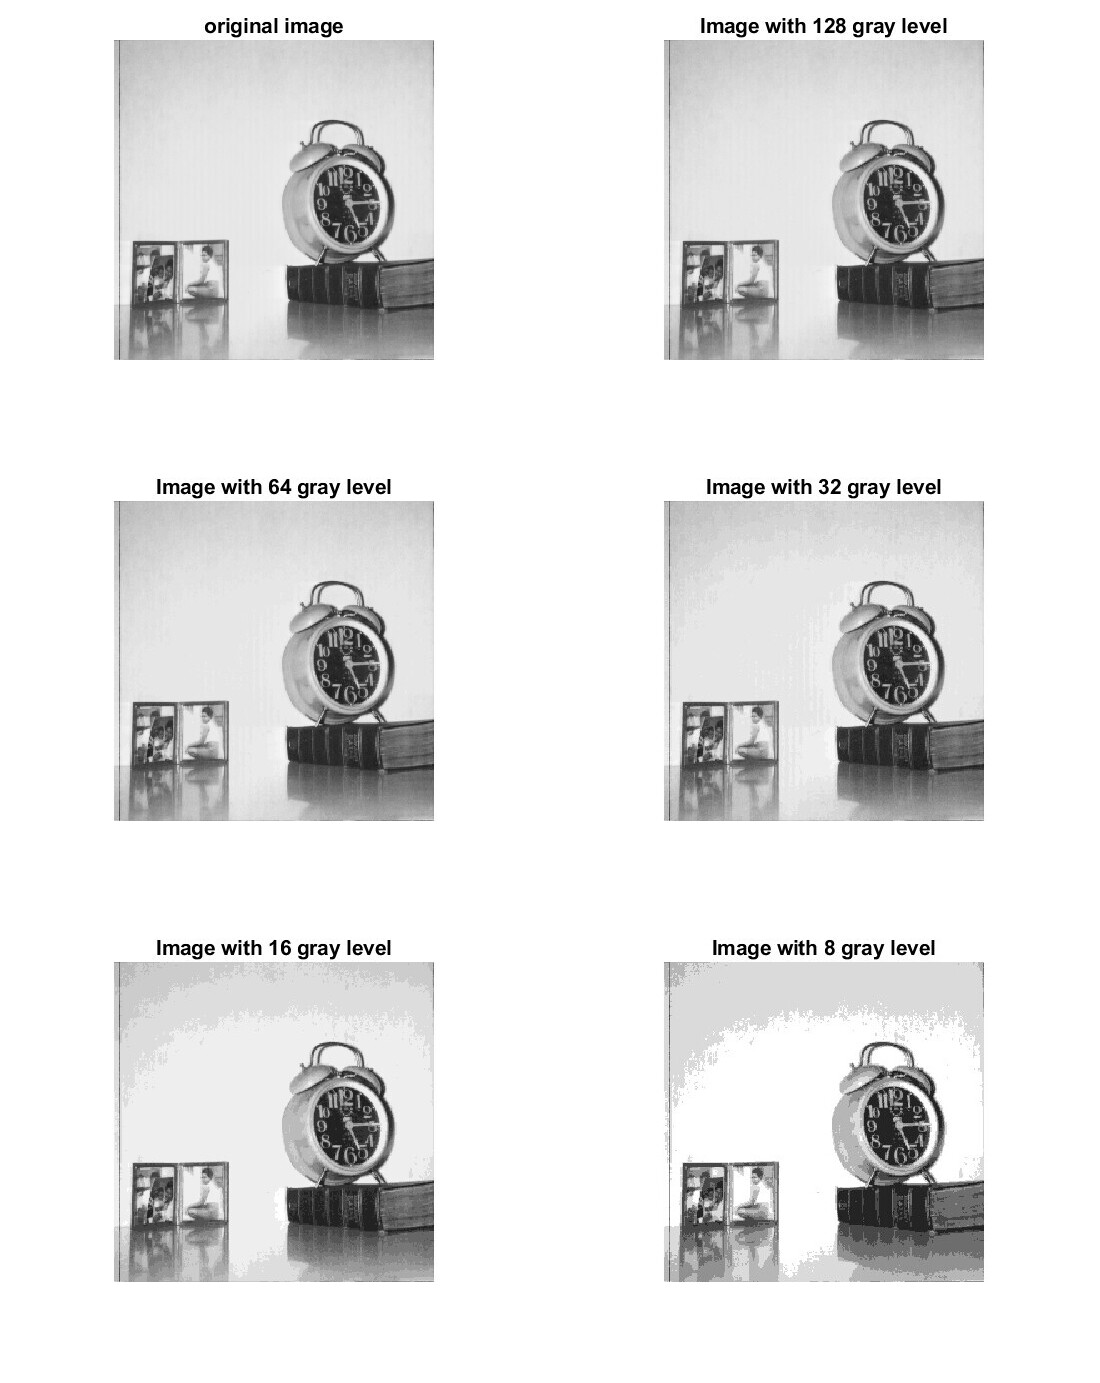
\includegraphics[width=.75\linewidth]{images/gray_scale_resolution.jpg}
    \caption{Ảnh xám với các độ phân giải mức xám khác nhau}
    \label{fig:gray_scale_resolution}
\end{figure}

\subsection{Phép toán giữa các điểm ảnh}

Các phép toán số học và logic trên hai ảnh được thực hiện trên từng điểm ảnh.
Các phép toán này chỉ thực hiện được nếu hai ảnh có cùng kích thước, nhưng nếu điều này không thỏa, ta vẫn có thể thực hiện các phép toán này trên vùng giao của hai ảnh. Nếu hai ảnh có kích thước $w_1 \times h_1$ và $w_2 \times h_2$ và giả sử gốc tọa độ của chúng giống nhau, vậy kết quả của phép toán trên hai ảnh này sẽ có kích thước $w \times h$, trong đó:

\begin{align}
    w &= \min (w_1, w_2) \\
    h &= \min (h_1, h_2)
\end{align}

\textbf{Phép cộng và trừ ảnh}

Cho hai ảnh $x_1$ và $x_2$ có vùng giao nhau có kích thước $W \times H$, $y$ là kết quả của phép toán giữa hai điểm ảnh, và các ảnh đều có độ phân giải mức xám N bit. Ta có các phép toán cộng và trừ giữa hai ảnh như sau:

\begin{align}
    y(i,j) &= \min \{ x_1(i,j) + x_2(i,j), 2^N \} \\
    y(i,j) &= \| x_1(i,j) - x_2(i,j) \|
\end{align}

Trong đó, $0 \leq i \leq H-1$ và $0 \leq j \leq W-1$.

Phép cộng ảnh có ứng dụng trong việc giảm nhiễu hình ảnh bằng cách lấy trung bình nhiều quan sát của cùng một khung hình. 
Phép trừ ảnh có ứng dụng trong việc phát hiện chuyển động, thông qua phân tích các điểm ảnh có giá trị khác không sau khi thực hiện phép trừ.

\textbf{Phép nhân và chia ảnh với một số}

Cho ảnh $x$ là ảnh thực hiện phép toán và ảnh $y$ là kết quả, có cùng kích thước và độ phân giải mức xám $N$ bit.
Phép nhân ảnh với một số $k$ được biểu diễn như sau:

\begin{equation}
    y(i,j) = k x(i,j) \quad (0 \leq i \leq H-1, 0 \leq j \leq W-1)
\end{equation}

Phép chia ảnh với một số tương tự như phép nhân, trong đó $|k| < 1$.

Phép nhân và chia các điểm ảnh với một số có thể được dùng để điều chỉnh độ sáng của một ảnh. Nhân các điểm ảnh với một số lớn hơn một sẽ làm sáng ảnh, và chia các điểm ảnh với một số lớn hơn mợt sẽ làm tối ảnh. Nhân (hoặc chia) các điểm ảnh với một số âm sẽ làm đảo màu của ảnh.

\textbf{Phép tích chập}: Tích chập rời rạc hai chiều giữa hai tín hiệu $x[n_1, n_2]$ và $h[n_1, n_2]$ là: 

$$y(n_1,n_2) = \sum_{k_1 = -\infty}^{+\infty} \sum_{k_2 = -\infty}^{+\infty} x(k_1,k_2) h(n_1-k_1, n_2-k_2)$$

Ở góc nhìn khác, phép tích chập hai chiều trong ảnh số chính là tính toán giá trị mới của điểm ảnh dưới dạng tổng có trọng số của các giá trị điểm ảnh trong một vùng lân cận nhất định xung quanh nó.

Tích chập có thể được sử dụng để thực hiện quá trình lọc tuyến tính.

\subsection{Một số loại loại nhiễu ảnh thường gặp}

\subsubsection{Nhiễu Gauss}

Nhiễu Gauss là nhiễu có hàm mật độ xác suất là phân phối Gauss. Nói cách khác, các giá trị mà nhiễu có thể nhận được phân bố theo Gauss.

Hàm mật độ xác suất $p$ của một biến ngẫu nhiên Gauss được cho bởi

$$p(z) = \frac{1}{\sqrt{2\pi} \sigma}e^{-(z-\bar{z})^2 / 2\sigma^2}$$

Trong đó $\sigma^2$ là phương sai và $\bar{z}$ là giá trị trung bình.

Các nguồn nhiễu Gauss chính trong ảnh số phát sinh trong quá trình thu thập. Cảm biến vốn có nhiễu do mức độ chiếu sáng và nhiệt độ của chính nó, đồng thời các mạch điện tử được kết nối với cảm biến cũng tạo ra phần nhiễu riêng của chúng.

\subsubsection{Nhiễu muối tiêu}

\textit{Nhiễu muối tiêu} hay còn gọi là \textit{nhiễu xung} là một dạng nhiễu đôi khi được thấy trên ảnh số. Nhiễu này có thể được gây ra bởi sự nhiễu loạn rõ rệt và đột ngột trong tín hiệu ảnh. Nhiễu này được thể hiện dưới dạng các điểm ảnh trắng và đen xuất hiện thưa thớt.

\begin{figure}[H]
    \centering
    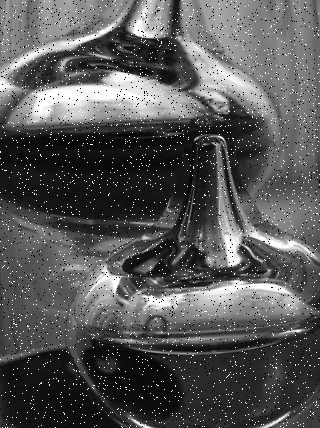
\includegraphics[width=0.5\linewidth]{images/salt_and_pepper_noise.png}
    \caption{Một ảnh với nhiễu muối tiêu}
    \label{fig:salt_and_pepper_noise}
\end{figure}

Hàm mật độ xác suất của nhiễu muối tiêu được cho bởi

$$p(z) = \left\{\begin{matrix}
P_a & z = a \\
P_b & z = b \\
0 & \text{khác} \\
\end{matrix}\right.$$

Trong đó $a = 0$ và $b = 255$ đối với ảnh mức xám 8 bit.

% \subsubsection{Nhiễu tuần hoàn}

% Một nguồn nhiễu tuần hoàn phổ biến trong ảnh là do nhiễu điện trong quá trình chụp ảnh. 
% Một ảnh bị ảnh hưởng bởi nhiễu tuần hoàn sẽ trông như một mẫu lặp lại đã được thêm lên trên ảnh gốc. 
% Trong miền tần số, loại nhiễu này có thể được coi là các xung rời rạc. 

% \begin{figure}[H]
%     \centering
%     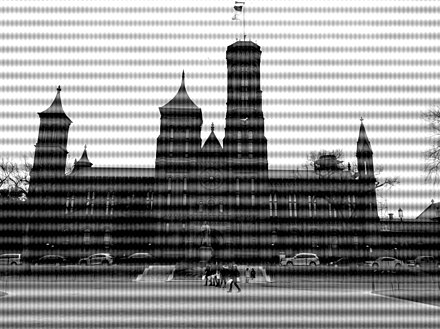
\includegraphics[width=0.75\linewidth]{images/periodic_noise.jpg}
%     \caption{Một ảnh với nhiễu tuần hoàn}
%     \label{fig:periodic_noise}
% \end{figure}

\subsection{Các loại bộ lọc}

Trong xử lý ảnh, một bộ lọc (hay còn gọi là kernel, ma trận tích chập, hay mặt nạ) là một ma trận có kích thước nhỏ so với kích thước ảnh cần được lọc, được ứng dụng trong việc làm mờ ảnh, sắc nét ảnh, phát hiện cạnh... 
Việc lọc ảnh được thực hiện bằng cách lấy tích chập giữa một bộ lọc và một ảnh. 
Một cách đơn giản, điểm ảnh ngõ ra là một hàm của các điểm ảnh ngõ vào lân cận (bao gồm cả chính nó).

Gọi $x(i,j)$ là ảnh gốc, $y(i,j)$ là ảnh sau khi lọc. Bộ lọc $h$ có kích thước $W_\text{filter} \times H_\text{filter}$. $S_{ij}$ là tập con của ngõ vào chứa các điểm lân cận xung quanh $(i,j)$:

$$S_{ij} = \begin{bmatrix}
x[i-m,j-n] & \cdots & x[i-m,j] & \cdots & x[i-m,j+n] \\
\vdots &  & \vdots &  & \vdots \\
x[i,j-n] & \cdots & x[i,j] & \cdots & x[i,j+n] \\
\vdots &  & \vdots &  & \vdots \\
x[i+m,j-n] & \cdots & x[i+m,j] & \cdots & x[i+m,j+n] \\
\end{bmatrix}, \quad m = \frac{H_\text{filter}}{2}, n = \frac{W_\text{filter}}{2}$$

Ta có biểu diễn tường minh của một số bộ lọc như sau:

Bộ lọc trung vị:

$$y(i,j) = \text{median}_{(s,t) \in S_{ij}}{\{x(s,t)\}}$$

Bộ lọc max:

$$y(i,j) = \max_{(s,t) \in S_{xy}}{\{x(s,t)\}}$$

Bộ lọc min:

$$y(i,j) = \min_{(s,t) \in S_{xy}}{\{x(s,t)\}}$$

Bộ lọc trung điểm:

$$y(i,j) = \frac{1}{2} \left ( \min_{(s,t) \in S_{xy}}[x(s,t)] + \max_{(s,t) \in S_{xy}}[x(s,t)]\right )$$
\section{Công cụ yêu cầu cho bài thí nghiệm}

\subsection{Phần mềm và phần cứng}

\textbf{Phần cứng}:
\begin{itemize}
    \item Bộ kit Raspberry Pi 3
    \item Màn hình, chuột, bàn phím (tùy chọn)
\end{itemize}

Ta có thể không cần dùng màn hình, chuột, bàn phím 
bằng cách tiền cấu hình tên người dùng, tên miền máy chủ, kết nối mạng... trước khi cài đặt 
và đăng nhập và điều khiển Raspberry Pi từ xa thông qua giao thức SSH hoặc VNC.

\textbf{Phần mềm}: Các phiên bản phần mềm và thư viện trong đề tài này là:
\begin{itemize}
    \item MATLAB R2023a trên máy tính
    \item Python 3.12 trên Raspberry Pi 3, với các module chính:
    \begin{itemize}
        \item numpy 1.26.4
        \item matplotlib 3.8.0
        \item opencv-python 4.9.0.80
        \item scipy 1.13.0
    \end{itemize}
\end{itemize}

\subsection{Giới thiệu bộ kit Raspberry Pi 3}

Các thông số kỹ thuật chính:

{ \centering
\begin{longtable}{rl}
\textbf{Vi xử lý:} & Broadcom BCM2837B0, Cortex-A53 64-bit SoC @ 1.4GHz \\
\textbf{Bộ nhớ:} & 1GB \\
\multirow{4}{*}{\textbf{Kết nối:}} & 2.4 GHz và 5 GHz WLAN \\
 & Bluetooth 4.2 BLE \\
 & Gigabit Ethernet over USB 2.0 \\
 & 4 cổng USB 2.0 \\
\multirow{4}{*}{\textbf{Video và âm thanh:}} & 1 x HDMI kích thước đầy đủ \\
 & Cổng display MIPI DSI \\
 & Cổng camera MIPI CSI \\
 & Ngõ ra stero 4 cực và cổng video composite \\
\multirow{3}{*}{\textbf{Multimedia:}} & H.264, MPEG-4 decode (1080p30) \\
 & H.264 encode (1080p30) \\
 & OpenGL ES 1.1, 2.0 graphics \\
\textbf{Hỗ trợ thẻ SD:} & Thẻ Micro SD cho việc khởi động hệ điều hành và lưu trữ dữ liệu \\
\multirow{2}{*}{\textbf{Nguồn:}} & 5V/2.5A DC qua kết nối micro USB \\
 & 5V DC qua header GPIO \\
\textbf{Nhiệt độ hoạt động:} & 0-50°C
\end{longtable}
}

\begin{figure}[H]
    \centering
    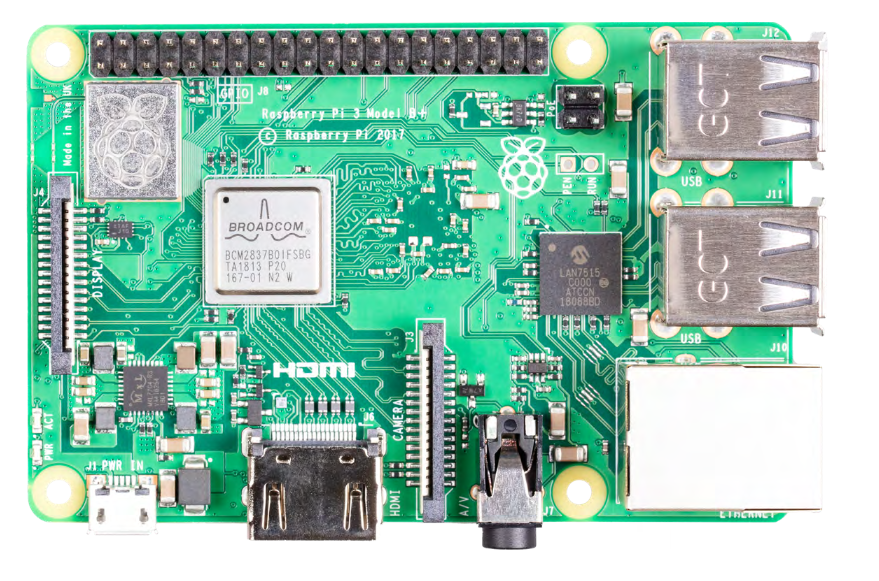
\includegraphics[width=0.75\linewidth]{../images/rpi3.png}
    \caption{Bộ kit Raspberry Pi 3 Model B}
\end{figure}
\section{Tiến hành thí nghiệm}

Các bước thí nghiệm chung:

\begin{enumerate}
    \item Thêm nhiễu cho ảnh bằng MATLAB
    \item Xử lý nhiễu bằng MATLAB trên máy tính và xứ lý nhiễu bằng Python trên Raspberry Pi 3
    \item Lấy kết quả MATLAB làm chuẩn để đánh giá kết quả giảm nhiễu ảnh trên Raspberry Pi.
\end{enumerate}

\begin{figure}[H]
    \centering
    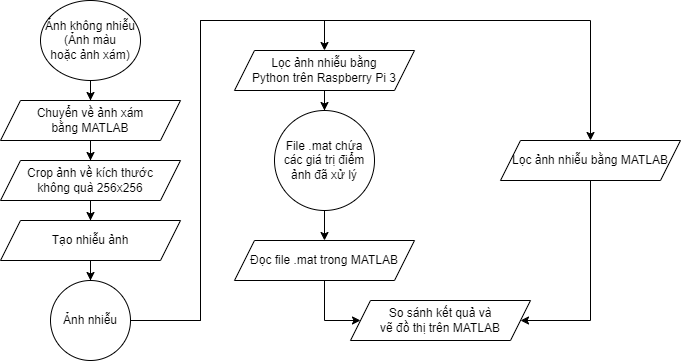
\includegraphics[width=\linewidth]{images/denoise_flowchart.png}
    \caption{Quy trình thí nghiệm}
\end{figure}

Để đánh giá hiệu quả của bộ lọc, ta tính sai số bình phương trung bình (mean square error, MSE) giữa ảnh gốc và ảnh đã lọc:

\begin{equation}\label{eqn:MSE}
    MSE = \frac{1}{WH} \sum_{i=1}^{H} \sum_{j=1}^{W} {(y_{ij} - x_{ij})^2}
\end{equation}

Trong đó, $W$ và $H$ là chiều rộng và chiều cao ảnh, $x$ là ảnh gốc và $y$ là ảnh đã lọc.

Ta tìm MSE bằng hàm \verb|mse| có sẵn của MATLAB.

\subsection{Triệt nhiễu ảnh muối tiêu}

\subsubsection{Tạo ảnh nhiễu muối tiêu trên MATLAB}

Ta đọc một ảnh gốc (ảnh màu hoặc ảnh xám), chuyển sang ảnh xám nếu cần, crop ảnh xuống $256 \times 256$ để thuận tiện cho việc xử lý. Cuối cùng, ta tạo nhiễu muối tiêu cho ảnh bằng hàm \texttt{imnoise} có sẵn của MATLAB.

\begin{lstlisting}[language=MATLAB]
figure, tiledlayout(1,2)

% Doc anh, chuyen sang anh xam, va crop anh neu kich thuoc lon hon 255
I = imread('dataset\4.1.03.tiff');
I = rgb2gray(I);
[rows, cols] = size(I);
size = [rows, cols];
if (rows > 256), I = imresize(I, [256 NaN]), end;
if (cols > 256), I = imresize(I, [NaN 256]), end;

% Luu anh xam da crop va hien thi anh
imwrite(I, 'images/salt_pepper_orig.bmp')
nexttile, imshow(I), title('Anh goc')

% Them nhieu muoi tieu voi mat do 0.05
J = imnoise(I, 'salt & pepper', 0.05);

% Luu anh da duoc tao nhieu va hien thi anh
imwrite(J, 'images/salt_pepper_noise.bmp')
nexttile, imshow(J), title('Anh nhieu muoi tieu 5%')
\end{lstlisting}

\begin{figure}[H]
    \centering
    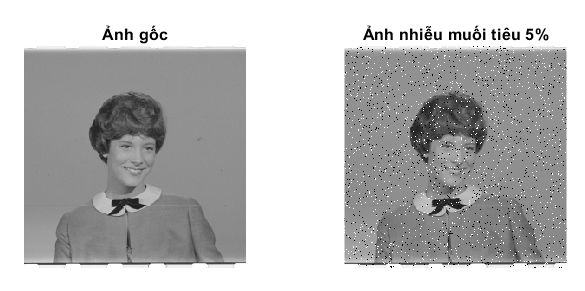
\includegraphics[width=.75\linewidth]{images/salt_pepper_noise_matlab.png}
    \caption{Tạo ảnh nhiễu muối tiêu trên MATLAB}
\end{figure}

\subsubsection{Lọc ảnh nhiễu muối tiêu bằng Python trên Raspberry Pi 3}

Các bước triển khai hàm lọc trung vị kích thước $3 \times 3$ trên Python như sau (Hình \ref{fig:median_filtering_algorithm}):

\begin{itemize}
    \item Padding cho ngõ vào: Để không bỏ sót các điểm ảnh ở rìa, ta cần padding cho ảnh ngõ vào. Vì bộ lọc có kích thước 3x3, ta cần padding 1 hàng zero cho rìa trên và dưới, và padding 1 cột zero cho rìa trái và phải.

    \item Tìm trung vị: Cho vòng lặp chạy qua từng điểm ảnh. Ở mỗi vòng lặp, xếp các điểm ảnh lân cận vào một mảng, sắp xếp mảng theo thứ tự tăng dần (hoặc giảm dần), và điểm ảnh ngõ ra sẽ là phần tử ở giữa của mảng đã sắp xếp.
\end{itemize}

\begin{figure}[h]
    \centering
    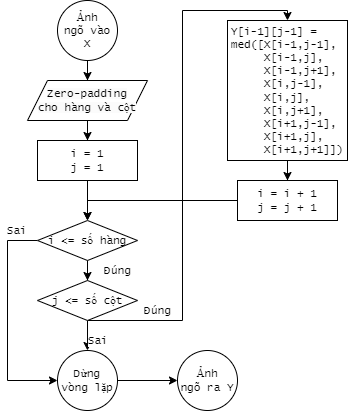
\includegraphics[width=.75\linewidth]{images/median_filtering_algorithm.png}
    \caption{Thuật toán lọc trung vị}
    \label{fig:median_filtering_algorithm}
\end{figure}

\begin{lstlisting}[language=Python]
import cv2
import numpy as np
import matplotlib.pyplot as plt
import scipy.io

# Doc anh nhieu muoi tieu
I = cv2.imread('output/salt_pepper_noise.png', cv2.IMREAD_GRAYSCALE)

# Ham loc trung vi kich thuoc 3x3
def medFilter3x3(X):
  nRows, nCols = X.shape

  # Padding cho anh ngo vao
  hpad = np.zeros((1, nCols))
  X = np.vstack((hpad, X, hpad))
  vpad = np.zeros((nRows+2, 1))
  X = np.hstack((vpad, X, vpad))
  
  # Lay trung vi bang cach sap xep theo thu tu lon dan
  # va chon phan tu thu 5 trong 9 phan tu
  Y = np.zeros((nRows,nCols))
  for i in range(1,nRows+1):
    for j in range(1,nCols+1):
      x = [X[i-1,j-1],
           X[i-1,j],
           X[i-1,j+1],
           X[i,j-1],
           X[i,j],
           X[i,j+1],
           X[i+1,j-1],
           X[i+1,j],
           X[i+1,j+1]]
      x = sorted(x)
      Y[i-1][j-1] = x[4]
  return Y

# Loc trung vi voi bo loc 3x3
J = medFilter3x3(I)

# Luu ket qua theo dinh dang cua MATLAB
scipy.io.savemat('output/salt_pepper_denoised_rpi3.mat', {"rpiDenoisedImg": J})
\end{lstlisting}

Kết quả chạy chương trình trên Raspberry Pi 3: 
Chương trình đọc ảnh nhiễu ngõ vào và xuất file \verb|salt_pepper_denoised_rpi3.mat| thành công để đưa vào MATLAB.

\subsubsection{So sánh kết quả với MATLAB}

Ta lọc ảnh bằng bộ lọc trung vị kích thước $3 \times 3$ với hàm \texttt{medfilt2()} có sẵn của MATLAB. 
Tiếp đến, ta vẽ ảnh đã lọc từ MATLAB và từ Raspberry Pi 3, 
đồng thời đánh giá các kết quả này dựa trên sai số bình phương trunb bình giữa ảnh đã lọc và ảnh gốc.

\begin{lstlisting}[language=MATLAB]
figure
tiledlayout(1,4)

% Doc anh xam goc va hien thi
I = imread('../output/salt_pepper_orig.png');
nexttile, imshow(I), title('Anh goc')

% Doc anh nhieu muoi tieu va hien thi
J = imread('../output/salt_pepper_noise.png');
nexttile, imshow(J), title('Anh nhieu muoi tieu')

% Loc trung vi voi bo loc 3x3 bang ham co san va hien thi
K = medfilt2(J, [3 3]);
nexttile, imshow(K), title(["Loc trung vi 3x3", "(MATLAB)"])
imwrite(K, '../output/salt_pepper_denoised_matlab.png')

% Doc ket qua loc trung vi 3x3 tu Raspberry Pi 3 va hien thi
load('../output/salt_pepper_denoised_rpi3.mat')
L = uint8(rpiDenoisedImg);
nexttile, imshow(L), title(["Loc trung vi 3x3", "(RPi 3)"])
imwrite(L, '../output/salt_pepper_denoised_rpi3.png')

% Sai so binh phuong trung binh giua anh goc va anh da loc
fprintf('MSE (MATLAB): %.4f\n', mse(I, K));
fprintf('MSE (RPi 3): %.4f\n', mse(I, L));
\end{lstlisting}

Kết quả chạy:

\begin{lstlisting}[style=output]
MSE (MATLAB): 3.8137
MSE (RPi 3): 3.8137
\end{lstlisting}

\begin{figure}[H]
    \centering
    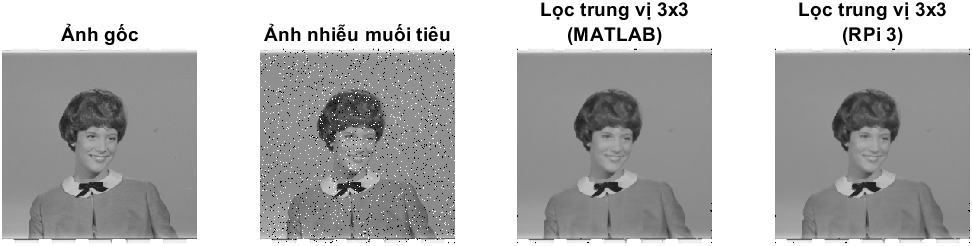
\includegraphics[width=1\linewidth]{images/salt_peper_compare.png}
    \caption{So sánh kết quả lọc trung vị từ Raspberry Pi 3 so với MATLAB}
\end{figure}

\textbf{Nhận xét:} Kết quả lọc trung vị từ Python trên Raspberry Pi hiệu quả tương đương MATLAB. 
Sai số bình phương trung bình giữa ảnh gốc và ảnh đã lọc trên Raspberry Pi 3 và trên MATLAB là giống nhau.

\subsection{Triệt nhiễu Gauss}

\subsubsection{Tạo ảnh nhiễu Gauss}

Ta đọc một ảnh gốc (ảnh màu hoặc ảnh xám), chuyển sang ảnh xám nếu cần, crop ảnh xuống $256 \times 256$ để thuận tiện cho việc xử lý. Cuối cùng, ta tạo nhiễu muối tiêu cho ảnh bằng hàm \texttt{imnoise} có sẵn của MATLAB.

\begin{lstlisting}[language=MATLAB]
figure
tiledlayout(1,2)

% Doc anh, chuyen sang anh xam, va crop anh neu kich thuoc lon hon 255
I = imread('dataset\4.2.01.tiff');
I = rgb2gray(I);
[rows, cols] = size(I);
size = [rows, cols];
if (rows > 256), I = imresize(I, [256 NaN]); end;
if (cols > 256), I = imresize(I, [NaN 256]); end;

% Luu anh xam da crop va hien thi anh
imwrite(I, 'images/gaussian_orig.bmp');
nexttile, imshow(I), title('Anh goc');

% Them nhieu Gauss voi trung binh 0, phuong sai 0.05
J = imnoise(I, 'gaussian');

% Luu anh da duoc tao nhieu va hien thi anh
imwrite(J, 'images/gaussian_noise.bmp');
nexttile, imshow(J), title('Anh nhieu Gauss mu=0, var=0.05');
\end{lstlisting}

\begin{figure}[H]
    \centering
    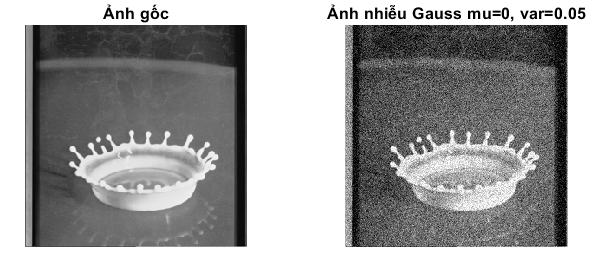
\includegraphics[width=.75\linewidth]{images/gaussian_noise_matlab.png}
    \caption{Ảnh nhiễu Gauss tạo từ MATLAB}
    \label{fig:gaussian_noise_matlab}
\end{figure}

Nếu không cung cấp thêm tham số, mặc định MATLAB sẽ tạo nhiễu Gauss trắng với trung bình $\mu = 0$ và phương sai hay công suất nhiễu $\sigma^2 = 0.01$.

\subsubsection{Lọc ảnh nhiễu Gauss bằng Python trên Raspberry Pi 3}

Với Python trên Raspberry Pi 3, ta lọc ảnh bằng bộ lọc Wiener với hàm \texttt{wiener()} của thư viện \texttt{scipy.signal}. 
Wiener là bộ lọc thông thấp một hình ảnh có giá trị cường độ bị suy hao bởi nhiễu cộng có công suất hằng. 
Với mỗi điểm ảnh, bộ lọc sẽ tìm trung bình và độ lệch chuẩn cục bộ trong một lân cận có kích thước được định sẵn.

Nếu không cung cấp thêm tham số kích thước bộ lọc và công suất nhiễu,
mặc định hàm \texttt{scipy.signal.wiener} sẽ ước lượng công suất nhiễu trước khi thực hiện quá trình lọc.

Tuy nhiên, cho tới phiên bản Scipy 1.13, hàm \texttt{wiener} không trả về giá trị được ước lượng của công suất.
Do đó ta tiến hành chỉnh sửa lại mã nguồn của hàm này như sau:

\begin{lstlisting}[language=Python]
from scipy.signal import correlate

def wiener(im, mysize=None, noise=None):
    im = np.asarray(im)
    if mysize is None:
        mysize = [3] * im.ndim
    mysize = np.asarray(mysize)
    if mysize.shape == ():
        mysize = np.repeat(mysize.item(), im.ndim)

    # Uoc luong trung binh cuc bo
    lMean = correlate(im, np.ones(mysize), 'same') / np.prod(mysize, axis=0)

    # Uoc luong phuong sai cuc bo
    lVar = (correlate(im ** 2, np.ones(mysize), 'same') /
            np.prod(mysize, axis=0) - lMean ** 2)

    # Uoc luong cong suat nhieu neu can
    if noise is None:
        noise = np.mean(np.ravel(lVar), axis=0)

    res = (im - lMean)
    res *= (1 - noise / lVar)
    res += lMean
    out = np.where(lVar < noise, lMean, res)

    return [out, noise]
\end{lstlisting}

Ta tiến hành thí nghiệm với hai trường hợp:
\begin{enumerate}
    \item (Mặc định) Không cung cấp tham số công suất nhiễu để phần mềm tự ước lượng giá trị này.
    \item Cung cấp trước tham số nhiễu ($\sigma^2 = 0.01$).
\end{enumerate}

\begin{lstlisting}[language=Python]
import cv2
import numpy as np
import matplotlib.pyplot as plt
import scipy.io

# Doc anh nhieu Gauss
I = cv2.imread('output/gaussian_noise.png', cv2.IMREAD_GRAYSCALE)

# Loc nhieu Gauss bang ham wiener() va luu ket qua
# Truong hop mac dinh (tu uoc luong cong suat nhieu)
[J_default, J_default_noise] = wiener(I, (3,3))
# Cung cap tham so cong suat nhieu var=0.01
[J_var0p01, J_var0p01_noise] = wiener(I, (3,3), 0.01)

# Luu ket qua loc theo dinh dang cua MATLAB
scipy.io.savemat('output/gaussian_denoised_rpi3.mat', 
                 {"J_default": J_default, 
                  "J_default_noise": J_default_noise,
                  "J_var0p01": J_var0p01})
\end{lstlisting}

Kết quả chạy chương trình trên Raspberry Pi 3: 
Chương trình đọc ảnh nhiễu ngõ vào và xuất file \verb|output/gaussian_denoised_rpi3.mat| thành công để đưa vào MATLAB.

\subsubsection{So sánh kết quả với MATLAB}

Ta lọc ảnh bằng bộ lọc Wiener với hàm \texttt{wiener2()} có sẵn của MATLAB. 
Nếu không cung cấp thêm tham số kích thước bộ lọc và công suất nhiễu,
mặc định MATLAB sẽ dùng cửa sổ lọc có kích thước $3 \times 3$, 
và ước lượng công suất nhiễu trước khi thực hiện quá trình lọc.

Tiếp đến, ta vẽ ảnh đã lọc từ MATLAB và từ Raspberry Pi 3, 
đồng thời đánh giá các kết quả này dựa trên sai số bình phương trunb bình giữa ảnh đã lọc và ảnh gốc.

\begin{lstlisting}[language=MATLAB]
fig = figure("Position", [0 0 800 500]);
tiledlayout(2,3)

% Doc anh xam goc va hien thi
I = imread('../output/gaussian_orig.png');
nexttile, imshow(I), title('Anh goc')

% Doc anh nhieu Gauss va hien thi
J = imread('../output/gaussian_noise.png');
nexttile, imshow(J), title(["Anh nhieu Gauss", "mu=0, var=0.05"])

% Loc nhieu Gauss bang ham wiener2 co san va hien thi
[K, noise] = wiener2(J);
nexttile, imshow(K), title(["Loc nhieu Gauss", "(MATLAB)"])
imwrite(K, '../output/gaussian_denoised_matlab.png')

% Doc ket qua loc nhieu Gauss tu Raspberry Pi 3 va hien thi
load('../output/gaussian_denoised_rpi3.mat')
L1 = uint8(J1_rpi3);
L2 = uint8(J2_rpi3);
nexttile, imshow(L1), title(["Loc nhieu Gauss", "(RPi 3, mac dinh)"])
imwrite(L1, '../output/gaussian_denoised_rpi3_default.png')
nexttile, imshow(L2), title(["Loc nhieu Gauss", "(RPi 3, var=0.01)"])
imwrite(L2, '../output/gaussian_denoised_rpi3_var_0p01.png')

% Cong suat nhieu uoc luong va sai so trung binh binh phuong
fprintf("Cong suat nhieu uoc luong (truong hop khong cung cap truoc tham so nhieu):\n");
fprintf('MATLAB: %.4f\n', K_noise);
fprintf('Raspberry Pi 3: %.4f\n', J_default_noise);
fprintf('\n');

fprintf('Sai so trung binh binh phuong giua anh goc va anh da loc:\n');
fprintf('MSE (MATLAB): %.4f\n', mse(I, K));
fprintf('MSE (RPi 3, default): %.4f\n', mse(I, L1));
fprintf('MSE (RPi 3, var=0.01): %.4f\n', mse(I, L2));
\end{lstlisting}

\begin{figure}[H]
    \centering
    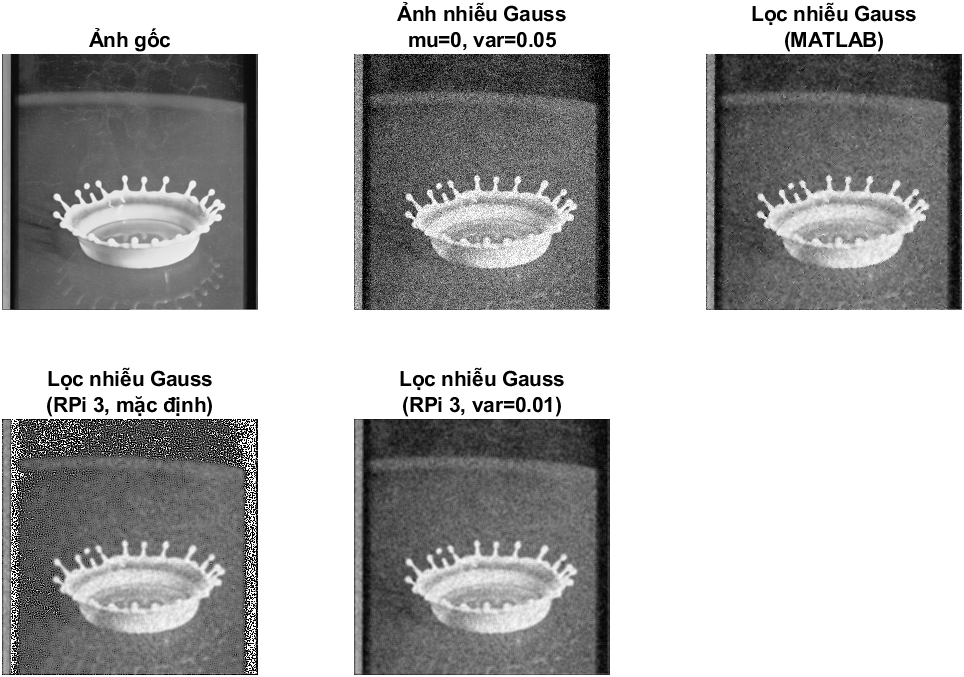
\includegraphics[width=1\linewidth]{images/gaussian_compare.png}
    \caption{So sánh kết quả lọc nhiễu Gauss từ Raspberry Pi 3 so với MATLAB}
\end{figure}

\textbf{Nhận xét}: Hàm \texttt{wiener2} của MATLAB ước lượng tốt công suất nhiễu (0.0105 so với 0.010), do đó cho kết quả lọc tương đối tốt. 

Khả năng ước lượng công suất nhiễu của thư viện scipy kém, dẫn đến kết quả lọc chưa tốt nếu không cung cấp tham số này. Với tham số công suất nhiễu được cung cấp, bộ lọc tỏ ra hiệu quả và kết quả lọc rất gần với kết quả của MATLAB và ảnh gốc.
\pagebreak
\section{Kết luận}

Đề tài đã thành công lọc được hai loại nhiễu cơ bản trong xử lý ảnh là nhiễu muối tiêu và nhiễu Gauss trên Raspberry Pi 3.
Kết quả cho thấy rằng phương pháp giảm nhiễu trên Raspberry Pi 3 có thể đạt được sai số thấp và kết quả gần với ảnh gốc. 
Trong phần lớn trường hợp, kết quả từ Raspberry Pi 3 không đạt được hiệu suất tốt như trên MATLAB.

Sự khác biệt trong kết quả giữa Raspberry Pi 3 và MATLAB có thể do nhiều yếu tố, 
bao gồm sự khác biệt trong thuật toán, cấu trúc phần cứng, hoặc việc triển khai thuật toán trên hai nền tảng khác nhau. 
Cải thiện có thể được thực hiện bằng cách tối ưu hóa thuật toán hoặc sử dụng phần cứng mạnh mẽ hơn để xử lý ảnh.

Đề tài này mở ra nhiều hướng nghiên cứu tiếp theo:
\begin{itemize}
    \item Tối ưu hóa các phương pháp giảm nhiễu để tăng hiệu suất và độ chính xác trên Raspberry Pi 3. 
    \item Nghiên cứu và áp dụng các phương pháp giảm nhiễu nhằm cải thiện kết quả. 
    \item Khảo sát và áp dụng các công nghệ phần cứng mới cho tác vụ giảm nhiễu hình ảnh.
    \item Nghiên cứu các phương pháp tự động điều chỉnh tham số để tối ưu hóa việc giảm nhiễu.
\end{itemize}

Tổng kết lại, việc giảm nhiễu hình ảnh bằng Raspberry Pi 3 là một đề tài quan trọng và có tiềm năng. 
Mặc dù đã đạt được một số kết quả tích cực, việc tiếp tục nghiên cứu và phát triển là cần thiết để cải thiện hiệu suất và độ chính xác của phương pháp trên nền tảng này.
\cleardoublepage
% \pagebreak
% \phantomsection
\addcontentsline{toc}{section}{Tài liệu tham khảo}

\nocite{*}
\printbibliography

\end{document}